% Created 2019-03-11 Mon 16:30
% Intended LaTeX compiler: pdflatex
\documentclass[11pt]{article}
\usepackage[utf8]{inputenc}
\usepackage[T1]{fontenc}
\usepackage{graphicx}
\usepackage{grffile}
\usepackage{longtable}
\usepackage{wrapfig}
\usepackage{rotating}
\usepackage[normalem]{ulem}
\usepackage{amsmath}
\usepackage{textcomp}
\usepackage{amssymb}
\usepackage{capt-of}
\usepackage{hyperref}
\author{Dhanush GA}
\date{\today}
\title{Land-Registry-Implementation}
\hypersetup{
 pdfauthor={Dhanush GA},
 pdftitle={Land-Registry-Implementation},
 pdfkeywords={},
 pdfsubject={},
 pdfcreator={Emacs 25.2.2 (Org mode 9.2.2)}, 
 pdflang={English}}
\begin{document}

\maketitle
\tableofcontents


\section{Implementation}
\label{sec:org872a95f}
The particular application has been developed using Blockchain technologies provided by Ethereum. The core of this application is handled by smart contracts. All the programming logic required to register users, lands and handle land transactions are written in smart contracts using the programming language called Solidity. This language is similar to javascript but helps us prevent critical errors like memory leaks, type errors etc. These smart contracts are compiled and then run on the Ethereum Virtual Machine (EVM). This Virtual Machine provides the resources for our smart contract to execute and its speciality is that it runs on the Ethereum Blockchain. Each state of a program is recorded as a transaction in the blockchain. 

To test this application, we run it in our local network using tools like Ganache and Truffle. Ganache simulates a local blockchain in our test environment by hosting a local blockchain and providing a few accounts to perform transactions. Truffle is used to compile the written smart contract and migrate (deploy) the contract to a running instance of a blockchain network. In our test network, we provide the address as that of the localhost (//127.0.0.1) and the port as 8545 (we can set the port value manually). After setting up all this to deploy our contract in a blockchain network, we could interact with our smart contract using ‘truffle console’ command. This command starts a console in which we could interact with our deployed contract and call the functions linked with our contract.

\begin{figure}[htbp]
\centering
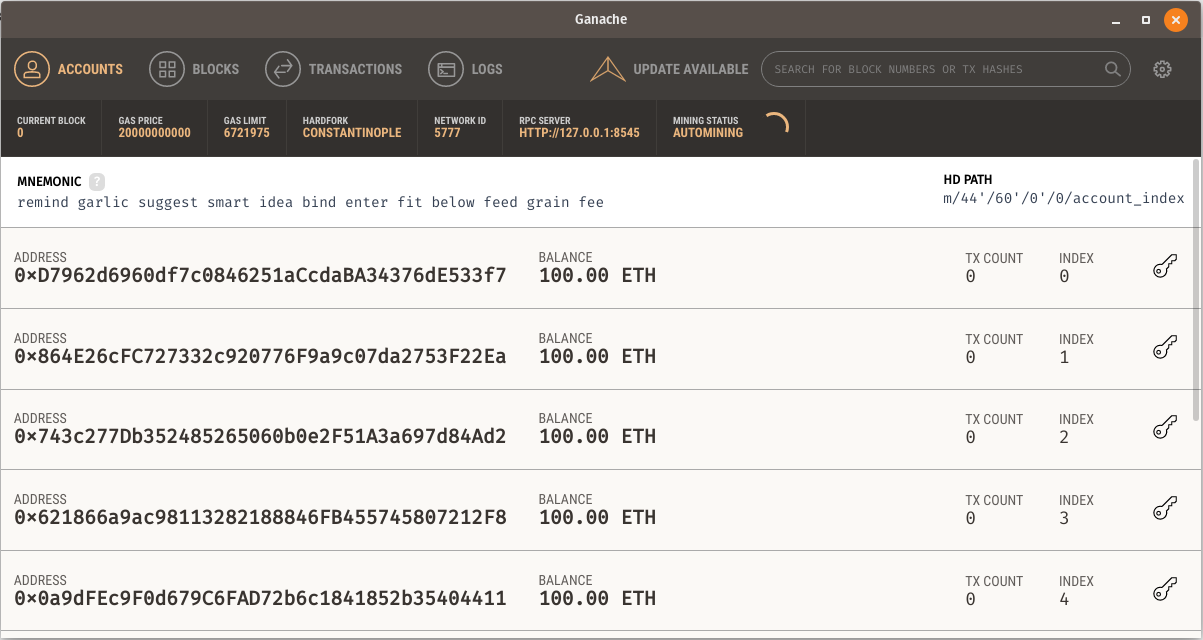
\includegraphics[width=.9\linewidth]{./ganache-interface.png}
\caption{Ganache User Interface}
\end{figure}

\subsection{User Registration}
\label{sec:org92f1944}
To register an user, we invoke registerUser() method. This function call receives user details and converts into a data structure holding user details. This data is then permanently stored in our blockchain.

\begin{figure}[htbp]
\centering
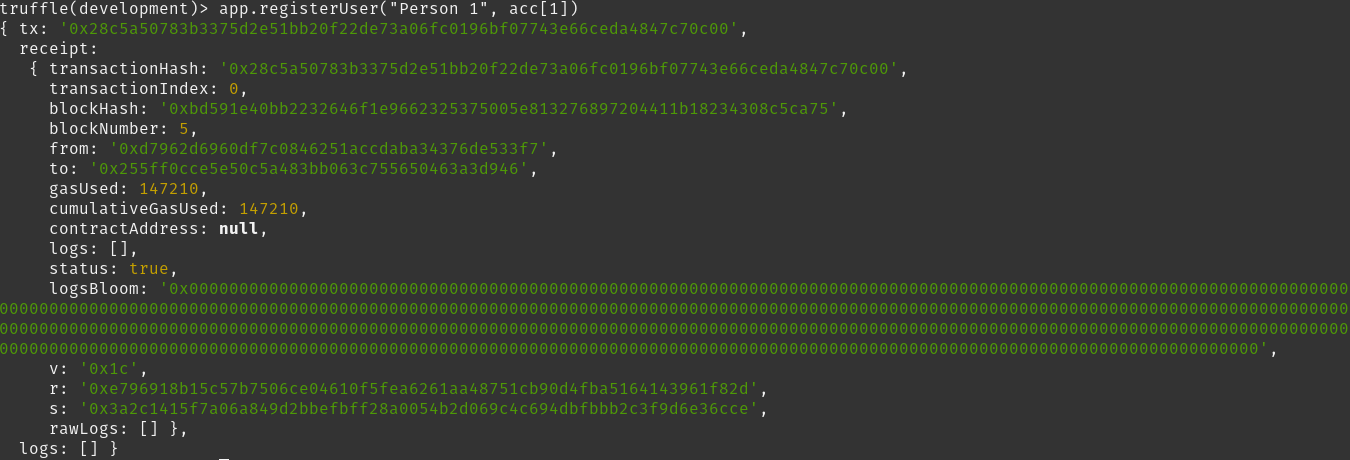
\includegraphics[width=.9\linewidth]{./register-person-1.png}
\caption{registerUser() method demonstration}
\end{figure}

\subsection{Land Registration}
\label{sec:org399147b}
Similar to user registration, we invoke registerLand() method to resgister a land. This method can only be used by privileged users (admin and regsistrar).
This data is converted to a data structure holding land details and then permanently stored in our blockchain. 

\begin{figure}[htbp]
\centering
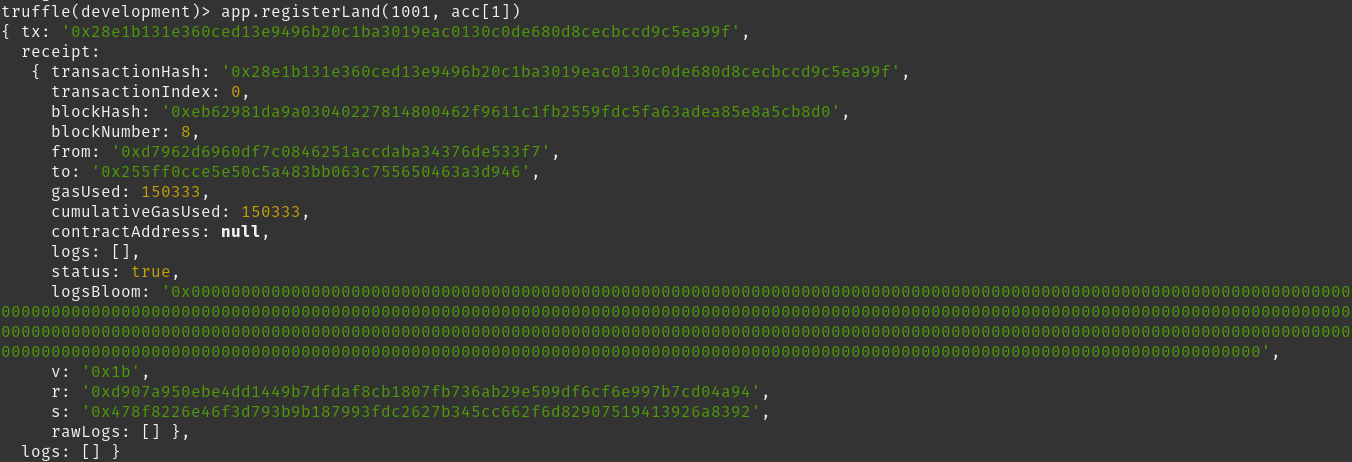
\includegraphics[width=.9\linewidth]{./register-land-1.png}
\caption{registerLand() method demonstration}
\end{figure}

\begin{figure}[htbp]
\centering
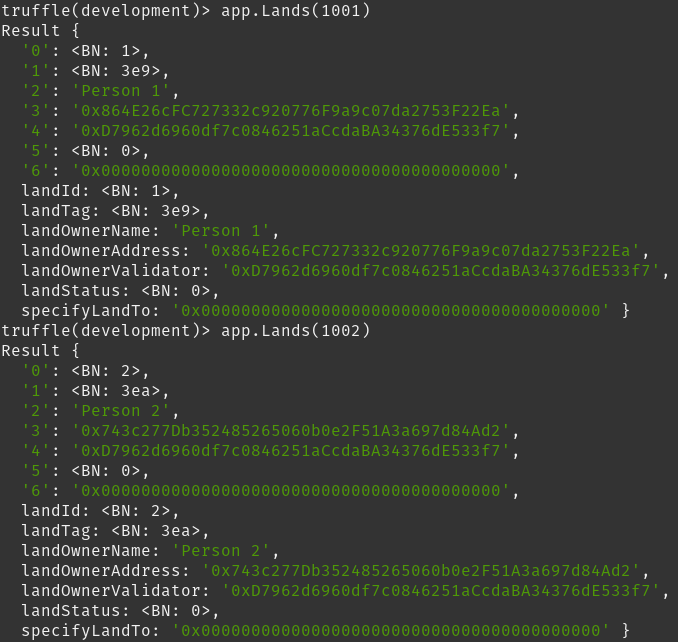
\includegraphics[width=.9\linewidth]{./land-details-1-2.png}
\caption{Land stored in Blockchain}
\end{figure}

\subsection{Land Transaction}
\label{sec:orgff0bfd9}
Land Transaction is carried out in this system only when the land is allowed to be sold. So, we include a method called chLandStatus() to allow the land owner to sell the land.

\begin{figure}[htbp]
\centering
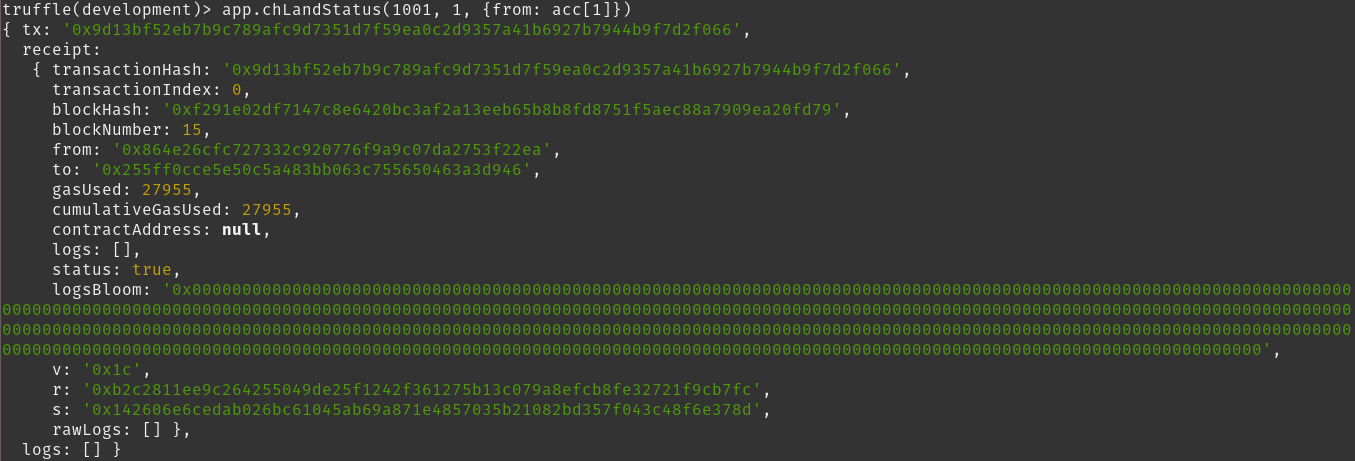
\includegraphics[width=.9\linewidth]{./change-land-status.png}
\caption{chLandStatus() method demonstration}
\end{figure}

If land is on sale \(\alpha\) \(\rightarrow\) \(\beta\), then invoking transactLand() method transfers the land from the land owner to the person invoking the method. Balance is deducted from the buyer's account and added to the seller's account. The land again changes to owned state. 

\begin{figure}[htbp]
\centering
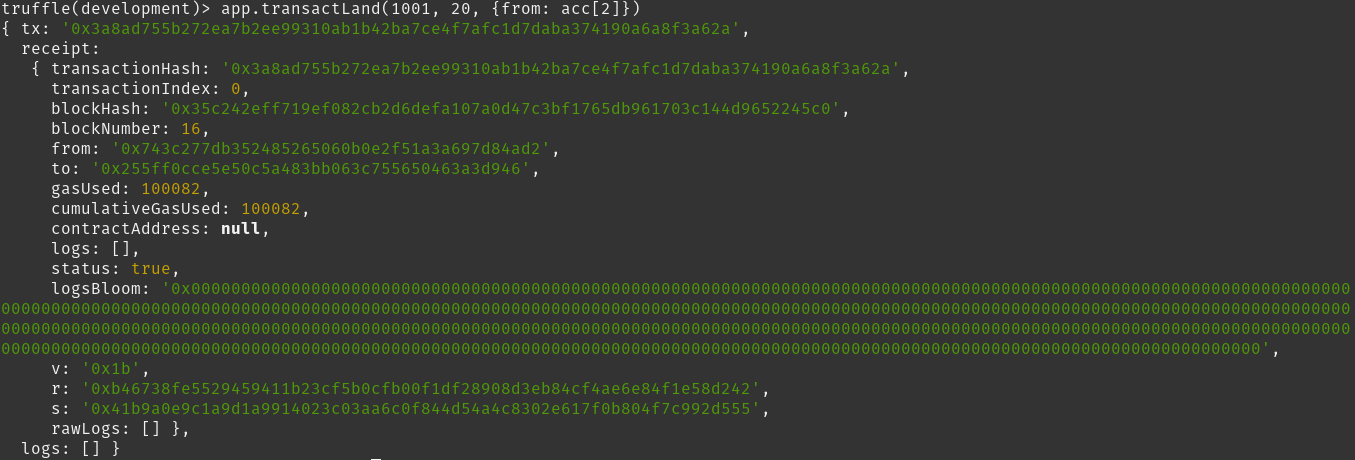
\includegraphics[width=.9\linewidth]{./transact-land.png}
\caption{transactLand() method demonstration}
\end{figure}

\begin{figure}[htbp]
\centering
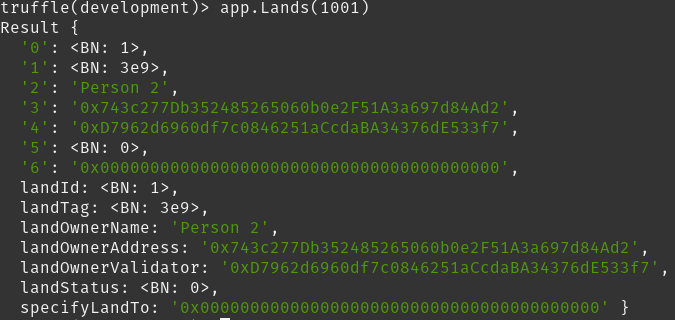
\includegraphics[width=.9\linewidth]{./land-status-after-transaction.png}
\caption{Land details after transaction}
\end{figure}

\begin{figure}[htbp]
\centering
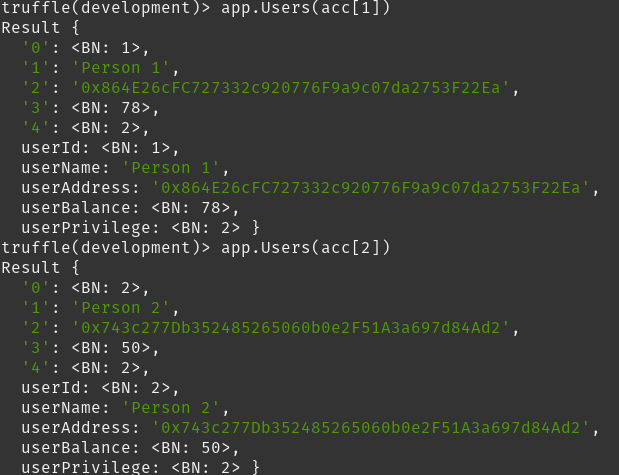
\includegraphics[width=.9\linewidth]{./user-status-after-transaction.png}
\caption{Updated user account details}
\end{figure}
\end{document}
